%% ---------------------------------------------------------------------
%% Copyright 2014, Thales, IGN, Rémi Cura
%% 
%% This file is the main file for the project of the short article on octree LOD
%% ---------------------------------------------------------------------

%% Inserting the settings and packages
	
%% ---------------------------------------------------------------------
%% Copyright 2014, Thales, IGN, Remi Cura
%% 
%% This file list the used package along description as well as other settings like used defined macro
%%
%%NOTE : 
%% ---------------------------------------------------------------------


%%Document structure :
	
	% 1 or 2 columns, chose one of the following
		%\documentclass[preprint,12pt,authoryear,twocolumn]{elsarticle}
		%\documentclass[preprint,3p,12pt,authoryear]{elsarticle}
		%\documentclass{rfpt}
		\documentclass{isprs}
		\usepackage{subfigure}
		\usepackage{setspace}
		\usepackage{geometry}
		\geometry{a4paper, top=25mm, left=20mm, right=20mm, bottom=25mm, headsep=10mm, footskip=12mm}
		
		%encoding
		\usepackage[utf8]{inputenc}
		
	%encoding
%		\usepackage[utf8]{inputenc}
	\usepackage{nameref}
	
	%math 
		\usepackage{amsmath}
		
		%\usepackage[url=false]{biblatex}
	%bibliogrpahy references style
		%%note : to remove URL from citations, comment line 371 of file elsarticle-harv.bst
		\bibliographystyle{isprs} 
		\usepackage{natbib} % necessary to control spacing
		\setlength{\bibsep}{1.5pt} % rcontrolling the spacing between references
		
	%hyperlink reference for inteligent pdf output 
 		\usepackage[pagebackref=true, pdftex]{hyperref}
		\hypersetup{colorlinks=true}

	%for the images
		\usepackage{graphicx}
		\DeclareGraphicsExtensions{.pdf,.png,.jpg}

%%Useful
	%adding more default colors%
		\usepackage[usenames,dvipsnames]{color}

	%allowing to display simple algorithm
		\usepackage{algorithm2e}
	%this package improve the spacing of letters : reduce the number of lines 
		\usepackage{microtype} 
		
	%allow to use SI unit with command
		\usepackage[squaren, Gray, cdot]{SIunits}

	%this package is buggy but provides way to include/exclude comment (used to generate a "debug" version of article)
		\usepackage{comment}
			%chose one of the two to show/hide comments
				\includecomment{proofreading}
				%\excludecomment{proofreading}
				
				\includecomment{illustrationInline}
				%\excludecomment{inline_illustration}
			
			%allow to modify the style of the commande : BUGGY : mess with subparapgraph command
				%\specialcomment{proofreading}{\begingroup\ttfamily\scriptsize\color{Orange}}{\color{black}\endgroup}
				%\specialcomment{proofreading}{\color{Orange}}{\color{black}}
			
	% add a \todo command to insert a todo and list it at the end of the document
		%% Note : chose between the 2 options to make todo inline or in margin
		%note : Change this package and switch to todonotes, more powerfull
		%\usepackage[superscript]{todo}
		%\usepackage[marginpar]{todo}  

	% another todo packages
		\usepackage[french,colorinlistoftodos]{todonotes}
		
	% defining a new command for emphas ein order to be able to desactivate it if necessary
		%%Note : the first option do somehting, chose the second one to do nothing (i.e. print text wihtout emphase)
		\newcommand{\myemph}[1]{\emph{#1}}
		%\newcommand{\myemph}[1]{#1}
	
	%defining new command for todo :
		% option to allow mutli lines in \todo[caption={Short note}
		% option to get arrow instead of lines : fancyline
		% option to precise author of todo : author=Xavier
		
		%redefining todo to add sub section number: 	
			%\newcommand{\ntodo}[2][]{\todo[#1]{\thesubsubsection{}. #2}}
		%use small line spacing :
			%\newcommand{\smalltodo}[2][]
			%{\todo[caption={#2}, #1]
			%{\begin{spacing}{0.5}#2\end{spacing}}}
		
		\newcommand{\mytodo}[2][]
		{\todo[size=\tiny,caption={#2}, #1, inline]
		{RC:\thesubsubsection{}. #2 }
		}
		
		%when a ref is missing or wrong	
		\newcommand{\todoref}[2][] 
			{\mytodo[color=blue!40, #1]
			{#2 }}
		
		%When a inside reference is missing or wrong
		\newcommand{\todorenv}[2][] 
			{\mytodo[color=yellow!40, #1]
			{#2 }}
		
		%When content need a rewrite
		\newcommand{\todorewrite}[2][] 
			{\mytodo[color=red!40, #1]
			{#2 }}
			
		%general todo
				\newcommand{\todoall}[2][] 
					{\mytodo[color=pink!40, #1]
					{#2 }}
					
		%When noting something
		\newcommand{\todonote}[2][] 
			{\mytodo[color=green!40, #1]
			{#2 }}
					
			%color option : blue : ref , green: note , red : rewrite
			
			
	%defining new command for image insertion
		%\usepackage{svg}
		
		\newcommand{\myimage}[3]
					{
					\begin{figure} [!h]
						\begin{center}
							\includegraphics[width=\linewidth,keepaspectratio]{#1}
							\caption{#2}  
							\label{#3}
							\end{center}
					\end{figure} 
					}
					
		\newcommand{\myimageFullPageHeight}[3]
						{
						\begin{figure*} [!h]
							\begin{center}
								\includegraphics[height=\textheight,keepaspectratio ]{#1}
								\caption{#2}  
								\label{#3} 
							\end{center}
						\end{figure*} 
						}
		\newcommand{\myimageFullPageWidth}[3]
								{
								\begin{figure*} [ht!]
									\begin{center}
										\includegraphics[width=\textwidth,keepaspectratio ]{#1}
										\caption{#2}  
										\label{#3} 
										\end{center}
								\end{figure*} 
								}
		
		\newcommand{\myimagelab}[3][] 
					{\begin{figure} [!h]
						\begin{center}
							\includegraphics[width=1\textwidth]{#1}
							\caption{#2}  
							\label{#3}
						\end{center}
					\end{figure} 
					}
					
		\newcommand{\myimageInline}[2]
					{
					\myimage{#1}{#2}
					}	 
		
	%defining a command to inser percent symbol
		%note : should be done using the siunitx package			
		\newcommand{\mypercent}{~\%}	
							
	%defining new command to change typo of remark area:
		\newcommand{\myremark}[1]{
		\color{black!80}
		#1
		\color{black!100}
		}
		%\todoall{trouver le bon style de typo pour les remarques}
	 
%% SETTINGS
	%show N level of hierarchy in table of content
		\setcounter{tocdepth}{3}%%chosing the numbe rof level in rable of contents. Default = 3
		
		\begin{proofreading}
			%show N level of hierarchy in table of content
				\setcounter{tocdepth}{4}%%chosing the numbe rof level in rable of contents. Default = 3
		%setting the size of margin in proof to help reduce page number
				%\usepackage[margin=1in]{geometry}
		\end{proofreading}
		
	
	
	

 
%opening
\title{ A Simple Ordering Solution for Efficient Geometrical Level Of Details on Lidar Point Cloud} 
\author{Rémi Cura  $^{AB}$, Julien Perret $^A$, Nicolas Paparoditis  $^A$}
\address{ $^A$  Universite Paris-Est, IGN, SRIG, COGIT \& MATIS, 73 avenue de Paris, 94160 Saint Mande, France\\
	first\_name.last\_name@ign.fr
	\\$^B$  Thales Training \& Simulation SAS, 1 rue du Général de Gaulle 95523 Cergy-Pontoise, France}


\keywords{RDBMS, point cloud, point cloud management, point cloud processing, filtering, indexing, compression, point cloud storage, point cloud I/O, point cloud generalisation, patch, point grouping}

\begin{document}

%\tableofcontents 
%remarques de Gildas :
%limitation ordering : le fait de stocker les points selon MidOc est très dommageable pour la localité des données, ce qui peut avoir un impact fort sur les accès mémoire.
%\\
%Le fait qu'on a déjà une acceleration spatiale sur les patch, et que donc on n en a pas besoin au niveau point n'est pas clair
%\\
%la partie sur la construction d'octree n'est pas forcément necessaire. Il faudrait mettre une grosse ref pour montrer qu'il y a eu enormement de travail dessus.
%\\
%Pour l'utilisation des LOD pour de la visu, il faudrait préciser que les critères peuvent être subtiles/visuel (par exemple screen space error : on fait le rendu, on mesure la taille de l'objet, puis on décide le niveau). Il faudrait préciser que ceci est compatible avec la methode proposée.
%\\
%Dans la conclusion, il faudrait parler de l'utilisation de niveaux de détails continus.

\maketitle 
%% Inserting the abstract
	%% ---------------------------------------------------------------------
%% Copyright 2014, Thales, IGN, Rémi Cura
%% 
%% This file is the abstract of the article
%% ---------------------------------------------------------------------


\begin{abstract} 
\begin{figure*}[t!]
	\begin{center}
		\fbox{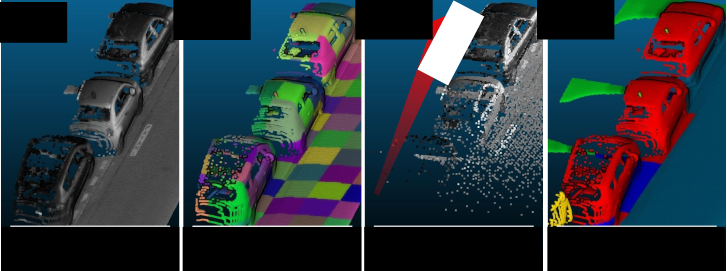
\includegraphics[width=\textwidth,keepaspectratio ]{./illustrations/banner_for_paper.png}}
		\caption{Data flow : starting from Lidar point cloud, we split it into patches, then reorder the patches to obtain free LOD (a gradient of LOD on this illustration). Lastly we use this ordering as feature for learning and efficient filtering} 
		\label{fig:banner_image}
		\end{center}
\end{figure*}
\newpage

This article introduce a new ordering for point cloud based on an octree, which allows, after a pre-computing phase to effortlessly get a representative geometric level of details of a point cloud, and even use the information as a crude classifier.

%sum um eachparts with 1-2 lines
\end{abstract}

%	\newpage

%% Inserting the introduction
	%% ---------------------------------------------------------------------
%% Copyright 2014, Thales, IGN, Rémi Cura
%% 
%% This file contains the introduction of article
%% ---------------------------------------------------------------------


\section{Introduction}
	\subsection{Problem} 
	 
		Point cloud data is becoming more and more common. Following the same trend, the acquisition frequency and precision are also increasing.
		Thus Lidar processing is clocking on the Big Data door.
		
		Yet the usage of point cloud data is also spreading and going out of the traditional user communities. 
		Lidar are now commonly used by non-specialized users. 
		
		
		For many usages, having the raw, complete point cloud is unnecessary, or even damageable.
		Thus we deal with a simpler version of a problem tat the vector community has faced for a long time : how to generalize point cloud, with data sets that are several order of magnitude bigger than usual vector data set?
		
		It is after all a problematic very common in data processing. Having a big data set, how to reduce its size while preserving its characteristics.
		It is the essence of compression for instance.
		
		Generalization is also more difficult when mixing data set with varying densities. For instance an aerial Lidar map augmented at certain places by terrestrial scanners, or vehicle-based Lidar acquisition, where the density varies with speed and scene geometry.
		
		Here we deal with a simplified version : given a point cloud, how to efficiently generate Level Of Detail (LOD for the remainder of this article) of this point cloud while preserving the geometric characteristic, without duplicating data.
		The key to LOD approach is efficiency. We accept to loose a part of the information in exchange of a massive reduction of data size. A solution using LOD must then by nature be efficient.
		
	%	\paragraph{}
	\subsection{Motivation}
		\begin{itemize}
			\item Point cloud : becoming common (why)
				Point cloud are becoming common because sensor are smaller, cheaper, easier to use. Point cloud from image (using Stereo Vision) are also easy to get with several mature structure from motion solutions.
				Point cloud complements very well images, Lidar point cloud allowing to avoid the ill-posed problem of stereo-vision, and providing key data to virtual reality.
			\item Growing data set + Multi sources 
				At such the size of data set are growing, as well as the number of dataset and their diversity.
			\item Why is it important (size of the industry) 
				The point cloud data are now well established in a number of industries, like construction, architecture, robotics, archaeology, as well as all the traditional GIS fields (mapping, survey, cultural heritage)
			\item PointCLoud users = specialist in processing, not informatics/storing 
				The LIDAR research community is very active. The focus of Lidar researchers is much more on Lidar processing and Lidar data analysis, or the sensing device, than on methods to render the data size tractable. 
		\end{itemize}   
		
	\subsection{state of the art}
		\todorewrite{when I have access to Zotero} 
		State of the art should include 
		\begin{itemize}
			\item what people do with point cloud ? (oosterom 2014)
		\end{itemize}
	\subsection{what's missing in biblio} 
		%limits of the already published articles
		
		Point cloud generalization methods are far from the subtlety of vector generalization ( // mettre des references).
		
		More generally, proposed methods usually focus on data compression and computing acceleration.
		
		Another common practice coming from Computer Graphics field is to compute an octree over the point cloud, then for each cell , compute a sub-sampled version of the point cloud.
		This allows to have simple and efficient Level of Detail , at the price of data duplication, and high sensibility to density variation.
		
		Moreover, all the method are specific and depend on a specific data structure that has to be stored extra to the point cloud data.Steaming from this the interoperability is non existent (moving from one software to another, one loose the data structure).
		
		We have then the classical and seemingly intractable trade-off between computing and storage : if we pre-compute a data structure, we have to store it extra. If we dot he computing on the fly, we may end up performing the same operations a lot's of time.
	
	\subsection{contribution}
		
		In this paper, we focus on simplicity, efficiency and re-use of existing and well established methods. All the methods are tested on Billion scale point cloud, and are open source for reproducibility test and reuse.
		We propose a simple method that enable portable computation free geometrical level of detail.
		The first contribution is that we propose to store the LOD information directly into the ordering of points rather than compute new sub-sampled point cloud for each LOD.
		Thus, the more we read points, the more precise of an approximation of the point cloud we get. If we read all the points, we have the original point cloud.
		
		The second contribution is a simple way to order points so that we have a varying geometric approximation of the point cloud when following this order.
		
		The third contribution is to use the ordering construction by-product as simple and free dimensionality descriptors, with usability demonstrated in a Random forest classification experiment.
			
		
	\subsection{plan of the article}
		The rest of this article is organized as follow :
		In the next section we present the methods.  
		In the section XX, we present some results and order of magnitude
		In the last section we discuss the results, the limitation and improvements of our solution.

%	\newpage

%% Inserting the Method part
	%% ---------------------------------------------------------------------
%% Copyright 2014, Thales, IGN, Rémi Cura
%% 
%% This file present the method of the article
%% ---------------------------------------------------------------------


\section{Method}
	\label{lod.sec:method}
	
	In this section, we first present the Point Cloud Server (section \ref{lod.method.PCS})(PCS \cite{Cura2015})
	that this article extends. Then we introduce the LOD solution that we propose 
	, which consists of reordering groups of points from less to more details (\ref{lod.method.order}), and then choose which LOD is needed.
	Although any ordering can be used, we propose a simple geometric one (\ref{lod.method:midoc}) which is fast and robust to density variation. 
	Furthermore, constructing this ordering produces a rough dimensionality descriptor (\ref{lod.method.dimdescriptor}). 
	This descriptor can be used in the PCS to perform density correction (\ref{lod.method.density}) and classification at the patch level (\ref{lod.method.classif}). This classification can be directly transferred to points, or indirectly exploited in a pre-filtering step.
	
	\subsection{The Point Cloud Server}
	\label{lod.method.PCS}
		\myimageHL{./illustrations/chap2/PCS/PCS}{Overall and storage organisations of the Point Cloud Server.}{lod.fig:PCS}{0.5}
		
		Our method strongly depends on using the Point Cloud Server described in \cite{Cura2015},
		therefore we introduce its principle and key relevant features (see figure \ref{lod.fig:PCS}).
		
		The PCS is a complete and efficient point cloud management system based on a database server that works on groups of points rather than individual points.
		This system is specifically designed to solve all the needs of point cloud users:
		fast loading, compressed storage, powerful filtering, easy data access and exporting, and integrated processing.
		
		The core of the PCS is to store groups of points (called patches) that are multi-indexed (spatially, on attributes, etc.), and represented with different generalisation depending on the applications.
		Points can be grouped with any rules.
		In this work, the points are regrouped spatially by cubes $1 \metre$ (Paris) or $50 \metre$ (Vosges) wide.
		
		All the methods described in this work are applied on patches.
		We propose is to reorder each patch following the MidOc ordering, allowing LOD and producing a dimensionality descriptor per patch. It can then be used to classify patches.
		
		We stress that our method used on any point cloud will provide LOD,
		but that using it with the PCS is much more interesting,
		and adds key feature such as spatial indexing, fast filtering, etc. 
 
 	 
	 	 
	\subsection{Exploiting the order of points}
		\label{lod.method.order}
		%\subsubsection{Principle} 
			
			\myimageHL{./illustrations/chap2/LOD/short_illustration_concept_lod/concept_Level_Of_Detail}{3 Geometrical Level Of Detail (LOD) for the same point cloud.
			Reading points from 1 to N gradually increases the details, because of the specific order of points (MidOc).}{lod.fig:lod-principle}{0.5}
			
			We propose to exploit the ordering of points to indirectly store LOD information.
			Indeed, whatever the format, be it file or database based, points ends up as a list, which is ordered.
			 
			The idea is then to exploit the order of this list, so that when reading the points from beginning to end, we get gradually a more accurate geometrical approximation of the point cloud (see figure \ref{lod.fig:lod-principle}). 
			 
			For instance, given list $L[P_1,..,P_N]$ of ordered points.
			Reading $P_1$ to $P_5$ gives a rough approximation of the point cloud, and reading another $16$ points ($P_1$ to $P_{21}$) is going to give a slightly better approximation. Reading points $1$ to $N$ is going to get the exact point cloud, so there is no data loss, nor data duplication.
		 
		%\subsubsection{Advantages}
			Using the point ordering as LOD results in three main advantages.
			%\paragraph{No on-line processing time}
			\paragraph{Implicit}
			Except a pre-processing step to write the point cloud following a given ordering, each time the user wants to get a Level Of Detail version of the point cloud, there is no computing at all (only data reading).
			This may not make a big difference for non-frequent reading, but in a context where the same point cloud is going to get used several times at several levels and by several users simultaneously (for instance Point Cloud as a Service), no processing time makes a big difference.
			%(See figure \ref{lod.fig:all_lod_illustration} for an example with LOD visualisation.) 		
		
			%\paragraph{No data duplication}
			\paragraph{No Duplication}
			Another big advantage is that exploiting point ordering does not necessitate additional storage.
			This is an advantage on low level. It saves disk space (no data duplication, no index file). Because the LOD information is embedded right within the point cloud, it is perfectly concurrent-proof, i.e. the point cloud and the LOD can not become out of sync.
			(Even in heavy concurrent Read/Write, a user would always get a coherent LOD).
			Lastly because the LOD only relies on ordering the original points, and does not introduces any other points or data, it avoids all precision-related issues that may come from aggregating.
			
			\paragraph{Portable}
			The last advantage comes from the simplicity of using the ordering. 
			Because it is already something that all point cloud tools can deal with (a list of points!), it is portable. Most softwares do not change the points order inside a cloud (See Section \ref{lod.result.os_softwares}).
			Even if a tool were to change the order, it would be easy to add the ordering number as an attribut (though slightly increasing the storage requirement).
			This simplicity also implies that adapting tools to exploit this ordering is very easy.
	
	
	\subsection{MidOc : an ordering for gradual geometrical approximation}
		\label{lod.method:midoc}
		\subsubsection{Requirements and hypothesis}
		\label{lod.method.midoc.hypothesis}
		The method exploits the order of points to store LOD information, so that the more points are read, the more detailed the result becomes.
		Obviously an ordering method that class the points from less details ($LOD_0$) to full details($LOD_\infty$) is needed.
		This ordering is in fact a geometric measure of point relevance, that is how well a point represents the point cloud (in a neighbourhood depending of the LOD).
		
		This ordering will be used by on different point clouds and for many applications, and so can not be tailored to one.
		As such, we can only consider the geometry (the minimal constituent of a point).
		Because of the possible varying-density point clouds, the ordering method also have to recreate a regular-ish sampling.
		
		Although many ordering could be used (for example, a simple uniform-random ordering),
		a suitable one would have low-discrepancy (that is be well homogeneous in space, see \cite{Rainville2012}), not be sensitive to density variations, be regular, be fast to compute and be deterministic (which simplify the multiuser use of the point cloud).
		
		We make two hypothesis that are mostly verified on Lidar point cloud.
		The first hypothesis ('disposable density') is that the density does not gives information about the nature of the object being sensed. 
		That is, depending on the sensing situation, some parts of the cloud are more or less dense, but this has nothing to do with the nature of the object sensed, thus can be discarded.
		The second hypothesis (low noise) is that the geometrical noise is low.
		We need this hypothesis because 'disposable density' forbids to use density to lessen the influence of outliers.
		
		A common method in LOD is to recursively divide a point cloud into groups and use the barycentre of the group as the point representing this group. The ground of this method is that the barycentre minimise the sum of squarred distance to the points.
		
		However such method is extremely sensible to density variation, and artificially creates new points. 
		
		\subsubsection{Introducing the MidOc ordering}
		
		\myimageHL{./illustrations/chap2/octree_ordering/octree_ordering_legend}{MidOc explained in 2D. Given a point cloud (Blue) and quad tree cells (dashed grey), the chosen point (green ellipse) is the one closest to the centre (black point) of the cell.}{lod.fig:midoc-principle}{0.5}
		
		We propose the re-use of well known and well proven existing methods that is the octree subsampling (for instance, the octree subsampling is used in \cite{Girardeau-Montaut2014}).
		An octree is built over a point cloud, then for each cell of the octree the LOD point is the barycentre of the points in the cell.  With this, browsing the octree breadth-first provides the points of the different levels.
		
		We adapt this to cope with density variation, and to avoid creating new point because of aggregation.   
		We name this ordering MidOc (Middle of Octree subsampling) for clarity, nonetheless we are probably not the first to use it.
		
		The principle is very simple, and necessitate an octree over the point cloud (octree can be implicit though).
		We illustrate it on Figure \ref{lod.fig:midoc-principle} (in 2D for graphical comfort).
		We walk the octree breadth-first.
		For each non-empty cell, the point closest to the cell centre is chosen and assigned the cell level,
		and removed from the available point to pick.
		The process can be stopped before having chosen all possible points,
		in which case the remaining points are added to the list, with the level $L_\infty$.
		
		The result is a set of points with level $(P,L_i)$.
		Inside one level $L_i$, points can be ordered following various strategies (see Section \ref{lod.method.intralevel}).
		
		Because each point is assigned a level, we can store the total number of points per level, which is a multi-scale dimensionality descriptor, see Section \ref{lod.method.dimdescriptor}).
		
		\subsubsection{Implementation}
		\label{lod.method.midoc.implementation}
		MidOc ordering is similar to octree building. Because Octree building has been widely researched, we test only two basic solutions among many possibilities.
		
		The first kind of implementation uses SQL queries. For each level, we compute the centres of the occupied cells using bit shifts and the closest point to these. Picked points are removed, and the process is repeated on the next level.
		It relies on the fact that knowing each point octree cell occupancy does not require to compute the octree (see Figure \ref{lod.fig:binary_coordinates_example}).
		
		The second implementation uses python with a recursive strategy. it only necessitates a function that given a cell and a list of points chose the point closest to the centre of the cell, then split the cell and the list of points for the next level, and recursively calls itself on this subcells with the sublists.
		
		A more efficient and simpler implementation is possible by first ordering the points following the Morton (Hypothesis : or Hilbert) curve, as  in \cite{Feng2014} (Section 2.5.1, page 37), in the spirit of linear octree.
		
		\subsubsection{Intra-level ordering}
		\label{lod.method.intralevel}
		
		\myimageHL{./illustrations/chap2/intralevel_ordering/intralevel_ordering_combined}{Several possible intra-level orders with various coverage from bad to good. Revert Morton and Revert Hilbert have offset for illustration.}{lod.fig:intralevel_ordering}{0.5}
		
		Inside one LOD points can be ordered with various methods.
		The intra-level ordering will have an impact if the LOD is used in a continuous way,
		and moreover may influence methods that relies on low-discrepancy.
		More precisely, if only a part of the points in a level are going to be used,
		it may be essential that they cover well the spatial layout of the totality of points.
		Several methods give this kind of coverage (see \cite{Rainville2012})
		
		Lets take the example where the goal is to find the plan that best fits a set of points
		and the method to do so in online (for instance it could be based on online robust PCA like in (\cite{Feng2013})).
		The plan fitting method reads one by one the points of a designated level $L_i$, and successively computes a better plan estimation.
		
		The Figure \ref{lod.fig:intralevel_ordering} presents some possible ordering. 
		If the plan detection method was applied on the Y ordering, it would necessitate a great number of points to compute a stable plan. For instance the first 16 points (1 column) would not permit to compute a plan.
		Similarly, if the point were ordered randomly, estimating a plan would still require lots of points, because uniform randomly chosen points are not well spread out (on the figure, the first 25 points are over represented in the upper left part).
		
		On the opposite, using a low discrepancy ordering like the Halton sequence makes the points well spread, while being quasi-random.
		Inverted space filling curves like the Morton or Hilbert curves also cover well space, at the price of being much more regulars.
		
		The Halton sequence ordering is obtained by generating a Halton sequence (nD points) and successively pick points closest to the Halton generated points.
		The revert Morton ordering and revert Hilbert ordering are the distance along Morton or Hilbert curve expressed in bit and read backward (with a possible offset).
		

	\subsection{Crude multi-scale dimensionality descriptor (MidOc by-product)} 
		\label{lod.method.dimdescriptor}
		\subsubsection{Principle}
		During MidOc building process, the number of chosen points per level can be stored.
		Each ordered patch is then associated with a vector of number of points per level $ppl=(N_{L_{1}},..,N_{L_{\text{max}}})$.
		The number of picked point for $L_i$ is almost the voxel occupancy for the level $i$ of the corresponding octree.
		Almost, because in MidOc points picked at a level do not count for the next Levels.
		Occupancy over a voxel grid has already been used as a descriptor (See \cite{Bustos2005}).
		However we can go a step further.
		For the following we consider that patches contain enough points and levels are low enough so that the removing of picked points has no influence.
		
		In theory for a level $L_i$, a centred line would occupy $2^{L_i}$ cells, a centred plan $4^{L_i}$ cells, and a volume all of the cells ($8^{L_i}$ cells).
		Thus, by comparing $ppl[L_i]$ to theoretical $2^{L_i}, 4^{L_i}, 8^{L_i}$ we retrieve a dimensionality indice  $Dim_{LOD}[i]$  about the dimensionality of the patch at the level $L$ (See Figure \ref{lod.fig:dim_descriptor}). 
		\myimageHL{"./illustrations/chap2/dim_descriptor/dim_descriptor"}{Voxel occupancy is a crude dimensionality descriptor: 3D line, surface or volume occupy a different amount of voxels.}{lod.fig:dim_descriptor}{0.5}
		This occupancy is only correctly estimated when the patch is fully filled and homogeneous. 
		However, we can also characterize the dimensionality $Dim_{LODDiff}$ by the way the occupancy evolves (difference mode).
		Indeed, a line occupying $k$ cells of an octree at level $L_i$ will occupy $2*k$ cells at the level $L_{i+1}$, if enough points.
		
		We stress that the information contained in $ppl$ is akin to a multi-scale dimensionality indice,
		with the scale being the level of the octree.
		For the rest of this work we consider that the dimensionality is roughly the same across level 
		 (which is entirely false in some case, see \ref{lod.result.dim_failure}).
		
		The Figure \ref{lod.fig:lod-common-objects} illustrate this. Typical parts of a street in the Paris dataset were segmented: a car, a wall with window, a 2 wheelers, a public light, a tree, a person, poles and piece of ground including curbs.
		\\
		Due to the geometry of acquisition and sampling, the public light is almost a 3D line, resulting in the occupation of very few octree cells.
		A typical number of points chosen per level for a public light patch would then be $(1,2,4,8,...)$, which looks like a $2^L$ function.
		A piece of ground is often extremely flat and very similar to a planar surface,
		which means that the points chosen per level could be $(1,4,16,64...)$, a $4^L$ function.
		Lastly a piece of tree foliage is going to be very volumetric in nature,
		due to the fact that a leaf is about the same size as point spacing and is partly transparent to laser (leading to several echo).
		Then a foliage patch would typically be $(1,8,64...)$ (if enough points), so a $8^L$ function.
		(Tree patches are in fact a special case, see \ref{lod.result.dim_failure}).
		
		\myimageHL{./illustrations/chap2/Objects/Objects_assembled}{All successive levels for common objects (car, window, 2 wheelers, light, tree, people, pole, ground), color is intensity for other points.}{lod.fig:lod-common-objects}{0.45}
				
		\subsubsection{Comparing crude dimensionality descriptor with covariance - based descriptors}
		
		A sophisticated per-point dimensionality descriptor is introduced in \cite{Demantke2014, Weinmann2015}, then used to find optimal neighbourhood size.
		A main difference is that this feature is computed for each point (thus is extremely costly to compute), and that dimensionality is influenced by density variation.
			 
		At the patch level, we do not need to find the scale at which compute dimensionality,	the descriptor is computed on the whole patch.
		
		
		This dimensionality descriptors ($Dim_{cov}$) relies on computing covariance of points centred to the barycentre (3D structure tensor), then a normalisation of covariance eigen values.
		As such, the method is similar, and has the same advantages and limitation, as the Principal Component Analysis (See \cite{Shlens2014} for a reader friendly introduction).
		It can be seen as fitting an ellipsoid to the points.
		
		First this method is sensible to density variations because all the points are considered for the fitting. 
		As opposite to our hypothesis (See Section \ref{lod.method.midoc.hypothesis}),
		this method considers implicitly that density holds information about the nature of sensed objects. 
		Second, this methods only fits one ellipse, which is insufficient to capture complex geometric forms. 
		Last, this method is very local and does not allow to explore different scale for a point cloud as a whole. Indeed this method is classically used on points within a growing sphere to extend the scale.
		
		However scale should be defined as the size of the features being analysed in sensed objects, and ot the scale of the neighbourhood of the centroid.
		
		We compute both dimensionality descriptor and then compare them for the Paris dataset.
		
		\subsubsection{crude dimensionality descriptor as a feature}

		Using the result of the MidOc ordering has the advantage of not necessitate extra computing,
		the patch being ordered with MidOc for LOD anyway.
		
		Moreover, because $x_1 \rightarrow (2^1)^x$,
		$x_2 \rightarrow (2^2)^x$, $x_3 \rightarrow (2^3)^x$ diverge very fast,
		we only need to use few levels to have a quite good descriptor.
		For instance, using $L=2$, we have $x_i=[4,16,64]$ , which are very distinguishable values, and don't require a total density above $70$ points per patch.  
		As long as the patch contains a minimal number of points, the descriptors is density and scale invariant.
		Lastly a mixed result (following neither of the $x_i \rightarrow (2^i)^x$ function) can be used as an indicator that the patch contains mixed geometry, either due to nature of the objects in the patch, or due to the way the patch is defined (sampling).
		
		Although it might be possible to go a step further and decompose a patch $ppl$ vector on the base of $x_i \rightarrow (2^i)^x, i \in [1..3]$, the direct and exact decomposition can't be used because the decomposition might depends on $L_i$. For instance a plane with a small line could appear as a plan for $L_1$ and $L_2$, and starts to appear differently over $L_3$ and higher level. In this case, an Expectation-Maximization scheme might be able to decompose robustly.
 
	\subsection{Excessive Density detection and correction}
		\label{lod.method.density}
		Lidar point cloud do not have a constant density, even if the acquisition is performed at a constant sensing rate, because the sensed object geometry (See Fig. \ref{lod.fig:irregular_sampling}).
		
		Important variation of density can be a serious issue for some processing methods. 
		For instance if millions of points are concentrated in a small volume,
		a processing method operating on fixed size volume may exceed the maximum memory of the system.
		Large density variation are also bad for performances in parallel environment.
		Indeed, efficient parallel computing may require that all the workers have about the same amount of work.
		One worker stumbling upon a very dense part of the point cloud would have much more points to process than the other workers.
		The figure \ref{lod.fig:density-correction} shows a place in the Paris dataset where the density is 5 times over the average value of this data set.
		In this context of terrestrial Lidar, this density peak is simply due to the fact that the acquisition vehicle stopped at this place
		, while continuing to sense data.
		
		The PCS coupled with LOD patches allows to quickly find abnormally high density.
		The PCS filters in few milliseconds the patch containing lots of points. This suffice for most applications.
		For a finer density estimation, we compute the approximate volume of the patch.
		For a level $L$, the $ppl[L]$ number of points multiplied by the theoretical cell size for this level gives an approximate volume (or surface) of the patch.
		The total number of points divided by this volume (surface) gives a finer volumetric (surface) density estimation.
		
		Then, correcting density consists of taking into account only the first $K$ points, where $K$ is computed to attain the approximate patch volume (surface).
		
		
	\subsection{Classification with the Point Cloud Server}
		\label{lod.method.classif}
		\subsubsection{Principle}
		
		We propose to perform patch classification using the Point Cloud Server and the previously introduced crude multi-scale dimensionality descriptor, along with other basic descriptors, using a Random Forest classifier.
		Following the position of the PCS towards abstraction, the classification is performed at the patch level and not at the point level. 
		This induces a massive scaling and speeding effect, at the cost of introducing quantization error.
		Indeed, compared to a point classification, a patch may contain points belonging to several classes (due to generalisation), yet it will only be classified in one class, thus the "quantization" error.
		
		Because patch classification is so fast and scales so well,
		the end goal can be however slightly different than for usual point classification.
		
		
		Patch classification can be used as a fast preprocess to another slower point classification,
		be it to speed it (an artificial recall increase for patch classification may be needed, see Figure \ref{lod.fig:recall-increase}), or to better a point classification.
		The patch classification can provide a rough classification.
		Based on that the most adapted point classifier is chosen 
		(similarly to Cascaded classifiers),
		thus improving the result of the final point classification.
		For instance a patch classified as urban object would lead to chose a classifier specialized in urban object, and not the general classifier.
		This is especially precious for classes that are statistically under-represented.
		 
		Patch classification may also be used as a filtering preprocess for applications that only require one class. 
		Many applications only need one class, and do not require all the points in it, but only a subset with good confidence.
		For this it is possible to artificially boost the precision (by accepting only high confidence prediction).
		For instance computing a Digital Terrain Model (DTM) only requires ground points.
		Moreover, the ground will have many parts missing due to objects,
		so using only a part of all the points will suffice anyway. 
		The patch classifier allow to find most of the ground patch extremely fast.
		Another example is registration.
		A registration process typically require reliable points to perform mapping and registration.
		In this case there is no need to use all points,
		and the patch classification can provide patches from ground and façade with high accuracy
		(for point cloud to point cloud or point cloud to 3D model registration),
		or patches of objects and trees (for points cloud to landmark registration).
		In other applications, finding only a part of the points may be sufficient, for instance when computing a building map from façade patches.
		
		
		
		Random Forest method started with \cite{Amit97shapequantization}, theorized by \cite{Breiman2001} and has been very popular since then. They are for instance used by \cite{Golovinskiy2009} who perform object detection, segmentation and classification. They analyse separately each task on an urban data set, thus providing valuable comparison. Their method is uniquely dedicated to this task, like \cite{Serna2014} who provide another method and a state of the art of the segmentation/classification subject.
		Both of this methods are in fact 2D methods, working on an elevation image obtained by projecting the point cloud. However we observe that street point clouds are dominated by vertical surfaces, like building (about 70\% in Paris data set). Our method is fully 3D and can then easily be used to detect vertical object details, like windows or doors on buildings.
		
		
		\subsubsection{Classification details}  
		\paragraph{Features}
		%\paragraph{Crude dimensionality descriptor}
		The first descriptor is $ppl$, the crude multi-scale dimensionality descriptor produced by the MidOc ordering (see Section \ref{lod.method.dimdescriptor}).
		We use the number of points for the level $[1..4]$. For each level $L$, the number of points is normalized by the maximum number of points possible ($8^L$), so that every feature is in $[0,1]$.
		
		%\paragraph{Other simple features}
		\label{lod.method.classification.other_feature}
		We also use other simple features that require very limited computing (avoiding complex features like contextual features). 
		Due to the PCS patch compression mechanism,
		min, max, and average of any attributes of the points are directly available.
		Using the LOD allows to quickly compute other simple feature, like the 2D area of points of a patch (points being considered with a given diameter). 
		
		\paragraph{Dealing with data set particularities}
		%\subsubsection{Analyzing data set classes}
		%\paragraph{Analysing class hierarchy} 
		The Paris data set classes are organized in a hierarchy (100 classes in theory, 22 populated).
		The rough patch classifier is not designed to deal with so many classes,
		and so a way to determine what level of hierarchy will be used is needed.
		We propose to perform this choice with the help of a graph of similarity between classes (See Fig. \ref{lod.fig:ppl-separator-power} and \ref{lod.fig:class-clustering-all-features}

		\label{lod.method.classification.spectral_layout}
		We first determinate how similar the classes are for the simple dimensionality descriptors, classifying with all the classes, and computing a class to class confusion matrix.
		This confusion matrix can be interpreted as an affinity between class matrix, and thus as a graph.
		We draw the graph using a spectral layout (\cite{Networkx2014}),
		 which amounts to draw the graph following the first two eigen vector of the matrix (Similar to Principal Component Analysis).
		Those two vectors maximize the variance of the data (while being orthogonal), and thus best explain the data.
		This graph visually helps to choose the appropriate number of classes to use.
		A fully automatic method may be used via unsupervised clustering approach on the matrix 
		(like The Affinity Propagation of \cite{Frey2007}).
		
		%\paragraph{Balancing the data set}
		Even when reducing the number of classes, the Paris dataset if unbalanced (some class have far less observations than some others).
		We tried two classical strategies to balance the data set regarding the number of observation per class.
		The first is under-sampling big classes : we randomly under-sample the observations to get roughly the same number of observation in every class.
		
		The second strategy is to compute a statistical weight for every observation based on the class prevalence. 
		This weight is then used in the learning process when building the Random Forest.
		
		\subsubsection{Using the confidence from the classifier} 
		\label{lod.method.classification.using_confidence}
		Contrary to classical classification method, we are not only interested in precision and recall per class, but also by the evolution of precision when prediction confidence varies.
		
		In fact, for a filtering application, we can leverage the confidence information provided by the Random Forest method to artificially boost precision (at the cost of recall diminution). We can do this by limiting the minimal confidence allowed for every prediction.
		Orthogonaly, it is possible for some classes to increase recall at the cost of precision by using the result of a first patch classification and then incorporate in the result the other neighbour patches. 
		
		We stress that if the goal is to detect objects (and not classify each point), this strategy can be extremely efficient.
		For instance if we are looking for objects that are big enough to be in several patches (e.g. a car).
		In this case we can perform the classification (which is very fast and efficient), then keep only highly confident predictions, and then use the position of predictions to perform a local search for car limits.
		The classical alternative solution would be to perform a per point classification on each point, which would be extremely slow.
		 
%	\newpage
	
%% Inserting the Result part
	%% ---------------------------------------------------------------------
%% Copyright 2014, Thales, IGN, Rémi Cura
%% 
%% This file present the result of the article
%% ---------------------------------------------------------------------


 \section{\label{sec:result}Result}
 	\subsection{introduction to all experiments}
 		We design and execute several experiments in order to validate all points that have been introduced in the "method" part.
 		First we prove that is it effectively possible to leverage points order, even using canonical open sources software out of the box.
 		Second we perform MidOc ordering on very large point cloud and analyse the efficiency, quality and applications of the results.
 		Third we use the number of points chosen in the MidOc ordering as a descriptors for a random forest classifier on two large data sets.
 		We analyse the potential of this free descriptors, and what it brings when used in conjunction to other simple descriptors.
	\subsection{Point Cloud server introduction}
		\subsubsection{principle}
			\paragraph{server}
				All the experiments are performed using a Point Cloud Server (article is being written, but a very detailed presentation is accessible \todoref{put reference to postgres presentation}).
				The key idea are that point clouds are stored inside a DBMS (postgres), as patch. Patch are groups of points along with some basic statistics about points in the group. Patch are compressed using various strategies.
				This organisation is based on the observation that in typical point cloud processing workflow, we never need a point alone, but more often a points and most likely its surrounding points.
			
			\paragraph{fast filtering}
				Each patch of points is then indexed in an R tree for most interesting attributes (obviously X and Y, but also time of acquisition, meta data, number of points, distance to source, etc.)
				
				Having such a meta-type with powerful indexes allows use to find points based on various criteria extremely fast. (order of magnitude : ms). 
				As an example we can find all points with given for a data set over 2 Billion points in a matter of milliseconds 
				 - between -1 and 3 meters high in reference to vehicle wheels
				 - in a given 2D area defined by any polygon
				 - close to a street called Rue Madame (according to IGN BDTopo)
				 - between 3 and 5 meters to the sensor position 
				 - not in buildings according to Open Data Paris building layer 
				 - acquired in the second passage of the vehicle a this place
				 - acquired between 8h and 8h10
		 
		    \paragraph{parallelism friendly}
				Cutting a point cloud into patches provides also a very easy parallel processing possibility, which we extensively use in our experiments.
		
			\paragraph{point cloud splitting}
				For our experiments we cut terrestrial Lidar point cloud into $1$ \cubic \meter cubes oriented on (North ,Est,Z) axis.
				We cut aerial lidar point cloud into $50^3$ \cubic \meter cubes.
				The choice of size is a compromise between speed, index size, patch size, typical feature size, etc.
				In fact the patch can be cut arbitrary, we chose this splitting for simplicity.
		
	\subsection{Data Set used}
		We use two data sets.
		\subsubsection{IQmulus data set}
			First \todoref{cite IQmulus data set}, an open source urban data set with varying density, singularities, and very challenging point cloud geometry.
			Data set is about 600 Millions points , over 12 kms of road. Points are typically spaced by 5cm to 0.2 cm. It is a multi echo laser (Riegl).
			We have access to a training set where every point is labeled in a hierarchy of 100 classes. The training set is only 12 millions points. Only 22 classes are represented.
			We will refer to this data set as Paris data set.
			
		\subsubsection{Vosges data set}
			We also use the Vosges data set, which is a very wide spread aerial data set of 6 billions points. 
			
			Density is much more constant to 10k pts/patch .
			We have access to a vector ground truth about surface occupation nature (type of forest), produced by the French Forest Agency.
			We will refer to this data set as the Vosges data set.
		
	\subsection{Exploiting the order of points}
		\subsubsection{experiment summary}
			In this first experiment we check that point cloud ordering is correctly preserved by common open source point cloud processing software.
			For this, we use a real point cloud, which we order by MidOc ordering. 
			We export it as a text file as the reference file.
			Then for each processing software, we read the reference file and convert it into another format, then check that the conversion didn't change the order. 
			The tree common open source software tested are CloudCompare, LasTools and Meshlab.
		\subsubsection{results}  
			All software passes test.
			We stress that even if software change order, it is still very easy to add the order as an attribute, thus making it fully portable.
			
	\subsection{MidOc : an ordering for gradual geometrical approximation}
		\subsubsection{experiment summary}
			In this experiment we first test ordering on typical street objects,then on terrestrial dataset to visually appreciate the fitness to use it for geometrical LOD.
			Then we compute MidOc for both our dataset and evaluate the trade-off between point cloud size and point cloud LOD.
			We briefly consider computing bottleneck.
			
			We demonstrate an immediate application of LOD for fast abnormal density detection and correction.
			Lastly as a proof of concept we stream 3D point cloud with various LOD to a browser.
		
		\subsubsection{visual evaluation}
			\paragraph{Visual evaluation on typical objects (ground, façade, car, pole, vegetation)}
				See fig XX \todorenv{put correct renv}
			
			\todorewrite{Visual results on aerial (Vosges).}
			\paragraph{visual evaluation aerial lidar}			
				See fig XX \todorenv{put correct renv}
		
		\subsubsection{size versus LOD tradeoff}
			We compute the size and canonical transfer time associated for a representative street and aerial point cloud.
			 	 
			 \begin{table}[ht]
				\centering
				\caption{ number of points per LOD, plus estimated transfer time with modern internet connection}
				\scriptsize 
				\begin{tabular}{|c|c|c|c|c|c}
				\hline Level & \shortstack{Typical \\ spacing(cm)} & \shortstack{ points \\ number(k)} & \shortstack{percent of \\ total size} & \shortstack{estimated \\ time Internet(s)}   \\
				\hline All & 0.2 to 5  & 1600 & 100 & 60 \\ 
				\hline 0 & 100 & 3 & 0.2 & 0.1 \\ 
				\hline 1 & 50 & 11.6 & 0.7 & 0.4 \\ 
				\hline 2 & 25 & 41 & 2.6 & 1.5 \\ 
				\hline 3 & 12 & 134 & 8.4 & 5 \\ 
				\hline 4 & 6 & 372 & 23 & 14 \\  
				
				\hline 
				\end{tabular} 
			\end{table}
			 
		\subsubsection{large scale computing}
		
			\paragraph{MidOc implementation} 
				We use 3 implementations of MidOc, two being pure plpgsql (postgreSQL script langage), and one python.
			\paragraph{Computing on very large dataset}
				We successively order all the Paris and Vosges data sets with MidOc, using 20 parallel workers, with a plpgsql implementation.
				The ordering is successful on all patches, even in very challenging areas where there are big singularities in density, and many outliers.
				The total speed is about 100 millions points/hour, which we consider as extremely slow.
				We briefly analyse performances, and conclude that data IO limits the number of efficient workers to 10, and that most of the time is actually not spend on computing, but on getting the points and writing them back.
				We note that a huge speed up is easily reachable by directly reading and writing binary patches (and not array of points), and use more reasonable C code instead of plpgsql script.
		\subsubsection{Fast abnormal density detection and correction}
			
			\myimage{./illustrations/density_detection_and_correction.png}{\label{fig:density-correction}Abnormal density detection and correction}
			
			\paragraph{density abnormality (peak)}
				Important variation of density can be a serious issue for some processing methods, or simply performances (especially in parallel environment). 
				The illustration shows a place where the density is 5 times over the normal value for this data set.
				In this context of terrestrial Lidar, this density peak is simply due to the fact that the acquisition vehicle stopped at this place, while continuing to sense data.
			\paragraph{Fast detection}
				We analyse the data set to find places of abnormally high density.
				It can be performed extremely fast at the patch level. (0.1 s for Vosges dataset, or a 2 Billion points urban dataset ). 
				The Top left image shows the number of points per \cubic \meter directly read from database, increasing from blue to yellow to red)
				In comparison, computing the density per point with neighbourhood is extremely slow (only for this 1.5 Million extract, 1 minute with CloudCompare,4x2.5GHz, 10cm rad) (top right illustration), and after the density is computed for each points, all the point cloud still need to be filtered to find abnormal density spot.
			
			\paragraph{simple correction}
				If the patch are ordered following MidOc, unneeded points are removed by simply putting a threshold on points per patch (bottom left, 1 to 5k points \per \cubic \meter , bottom right , 5k to 24 k pts \per \cubic \meter). It considerably reduces the number of points (-33%).
			
				
		\subsubsection{LOD stream}
			As a proof of concept we stream points from the data base to a browser \todoref{citer ITowns}.
			For this experiment we only stream a given number of points per patch, which allows to accelerate greatly data loading.
			
			
			limitation
			However we didn't use the LOD to perfom a distance-dependend density :  display patch with varying LOD given their distance to camera.
			
			??(parler du stream de patch dans itowns?)??
			limitation = have to put the whole patch in memory, even when getting only few points.
			Conclusion : as is : interesting when bandwidth limited.  
			
			
	\subsection{using the ordering by-product as a crude dimensionality descriptor}
		\subsubsection{experiment summary}
			For each patch, we store the associated number of points chosen per level while computing MidOc ordering. We call this descriptor $points_per_level$.
			
			This dimensionality descriptor alone cannot be used to perform sophisticated classification, because many semantically different objects have similar dimension (for instance, a piece of wall and of ground are dimensionally very similar, yet semantically very different).
						
			We descriptors we use are (P : for Paris , V : for Vosges: 
			  - $points_per_level$, level 1 to 4 (P+V)
			  - average of intensity (P+V)
			  - average of $number_of_echo$ (P+V)
			  - average of height regarding laser origin(P)
			  - average Z (V)
			  - patch height (P)
			  - area of $patch_bounding_box$ (P) : 
			 
		\subsubsection{choosing classes in class hierarchy}
			Choosing which level of the class hierarchy uses depends on data set and applications.
			
			\paragraph{canonical classification}
			
				In a canonical classification perspective, we have to strongly reduce the number of classes if we want to have significant results.
				However reducing the number of class (i.e use a higher level in the classes hierarchy) also means that classes are more heterogeneous.
				
				We planned to automatically chose classes by clustering the confusion matrix (understood as an affinity matrix for the clustering method), but the wide difference in statistical weight and the variance of predictions for small classes deterred us from this approach.
				
				Both data set are extremely unbalanced (factor 100 or more frequent). Thus our simple and direct Random Forest approach is ill suited for dealing with extremely small classes. (we would need to use some kind of cascading or appropriate one versus all learning).
				
				For Vosges data set a short analysis convince us to use 3 classes : Forest, Land, and other, on this three classes, the Land class is statistically overweighted by the 2 others.	
			
				For the Paris data set, the representation of classes is very ill-balanced.
				Keeping only the class above 0.5 \% reduce the number of classes to 12.
				The class under-represented have a strong variability in result.
				Also, some class cannot be properly defined without context (e.g. the side-walk, which is by definition the space between building and road, hence is defined contextually).
		 	
			The main sources of error is that many patches contains mixes of classes, especially for class of small objects. 
			\paragraph{balancing data set}
				 We abandoned the under-sampling approach because we think that in this case it can introduce significant bias.
				 The urban objects are very diverse, and so each class is quite heterogeneous. Thus, by under-sampling, we artificially increase the variability of the results.
				 We prefer the approach with weight, even if it performs poorly when the difference beteen classes is to large.
				
			\paragraph{classifying}
				
				The computing time (10 fold, tree = 100) is between one and 20 minutes depending on the number of observation and the number of classes.
				
				We note that most errors are on patches with mixed contents.
				We perform a analysis of error on Vosges dataset and we remark that the error seems to be significately correlated to distance ot borders.
				
				\todo{put results on vosges, all classes }
				\todo{put results on vosges, 3 classes }
				
				
				\todo{put results on Paris, all classes }
				\todo{put results on Paris, main classes }
								
				 
				 
		
 
%	\newpage

%% Inserting the Result part
	%% ---------------------------------------------------------------------
%% Copyright 2014, Thales, IGN, Rémi Cura
%% 
%% This file is the Discussion of the result of the article
%% ---------------------------------------------------------------------


 \section{ Discussion }
	 \label{sec:discussion} 
	 
	 \subsection{Point cloud server}
	\label{par:pointcloudserver-limitation}
	We refer the reader to \cite{Cura2014} for an exhaustive analyse of the Point Cloud Server.
	Briefly, the PCS has demonstrated all the required capacitites to manage point clouds and scale well.
	To the best of our knowledge the fastest and easiest way to filter very big point cloud using complex spatial and temporal criteria, as well as natively integrate point cloud with other GIS data (raster, vector).
	The main limitation is based on the hypothesis than points can be regrouped into meaningful (regarding further point utilisation) patch. If this hypothesis is false, the PCS loose most of its interest.
	 
		 
	\subsection{Exploiting the order of points}
	From a practical point of view, implicitly storing the LOD using the point ordering
	seems to be estremely portable. Most softwares would not change the order of points.
	For those who might change the order of points, 
	it is still very easy to add the order as an attribute, thus making it fully portable.
	However, this approach has two limitations.
	The first limitation is that the order of point might already contains precious information. 
	For instance with a static Lidar device,
	the acquisition order allows to reconstruct neighbourhood information.
	The second limitation is that an LOD ordering might conflict with compression.
	Indeed ordering the points to form LOD will create a list of points were successive points are very different. Yet compressing works by exploiting similarities.
	A software like LasTool using delta compressing might suffer heavily from this. 
			 
	 \subsection{MidOc : an ordering for gradual geometrical approximation}
	 	We stress that the LOD are in fact almost continuous (as in the third illustrations of \ref{fig:banner_image}).
	 	\myimage{./illustrations/Objects/Objects_assembled.jpg}{All successive levels for common objects (car, window, 2 wheelers, light, tree, people, pole, ground), color is intensity for other points.}{fig:lod-common-objects} 
		 	
		MidOc is a way to order points based on their importance. In MidOc,
		the importance is defined geometrically.
		Yet specific applications may benefit from using other measure of importance, 
		possibly using other attributes than geometrical one,
		and possibly using more perceptual-oriented measures.
		
		MidOc relies on two hypothesis which might be false in some case. 
		Indeed, variation of density may be a wanted feature
		(e.g. stereovision, with more image on more important parts of the object being sense).
		Again the low geometrical noise hypothesis might be true for Lidar, but not for Stereo vision 
		or medical imaging point cloud. However in those case denoising methods may be applied before computing MidOc.

	\subsubsection{Applications}
		MidOc ordering might be of use in 3 types of applications. First it can be used for graphical LOD, as a service for point cloud visualisation.
		Second the ordering allows to correct density to be much more constant.
		Complex processing methods may benefits from an almost constant density, or for the absence of strong density variation.
		Third the ordering can be used for point cloud generalisation,
		as a service for processing methods that may only be able to deal with a fraction of the points. 
		
		The illustration \ref{fig:visual_LOD_left_right} gives visual example of LOD result and how it could be used to vary density depending on the distance to camera. 
		Figure \ref{fig:lod-common-objects} also gives visual examples for common objects of different dimensionality.
		It is visually clear that the rate of increase of points from LOD 0 to 4 for floor lamp (1D) window (2D) and tree (3D) is very different.
		Small details are also preserved like the poles or the antenna of the car. preserving those detail with random or distance based subsampling would be difficult.
		
		 
	\subsubsection{Implementation}
			%\subsubsection{Efficiency and performance}
		\label{subsubsec:bit_coordinates}
		Octree construction may be avoided by simply reading coordinates bitwise in a correctly centred/scaled point cloud.
		We centre a point cloud so that the lowest point of all dimension is $(0,0,0)$, and scale it so that the biggest dimension is in $[0,1[$.
		The point cloud is then quantized into $[0..2**L-1]$ for each coordinate.
		The coordinates are now integers, and for each point, reading its coordinates bitwise left to right gives the position of the point in the octree for level of the bit read.
		This means performing that this centring/scaling/quantization directly gives the octree. Moreover, further operations can be performed using bit arithmetic, which is extremely fast.
		\myimage{./illustrations/LOD/principle_of_binary_coordinate.png}{Principle of binary coordinates for a centered, scaled and quantized point cloud.}{fig:binary_coordinates_example}
		
		On this illustration the point $P$ has coordinates $(5,2)$ in a $[0,2^3-1]^2$ system. Reading the coordinates as binary gives $(b'101',b'010')$.
		Thus we now that on the first level of a quad tree, $P$ will be in the right (x=$b'1xx'$) bottom (y=$b'0yy'$) cell.
		For the next level, we divide the previous cell in 2, and read the next binary coordinate. $P$ will be in the left (x=$b'x0x'$) up (y=$b'y1y'$) cell. There is no computing required, only bit mask and data reading.
			
		Regarding implementation, the three we propose are much too slow, by an order of magnitude to be easily used in real situation. We stress however that the slowness comes from ineficient data manipulation, rather than from the complexity of the ordering. 
		It may also be possible to use the revert Hilbert ordering to directly compute MidOc.
		Furthermore, octree construction has been commonly done on GPU for more than a decade.
	 \subsubsection{Size versus LOD trade-off}
		 \label{point-cloud-server-troughput}
		 The table \ref{tab:lod-size-time} shows that using the level 3 may speed the transfer time by a 10 factor.
		 The point cloud server throughput is about 2-3 \mega $byte$ \per \second  (monoprocess),  sufficient for an internet troughput, but not fast enough for a LAN 10 \mega $byte$ \per \second.
		 This relatively slow troughput is due to current point cloud server limitation (cf \ref{par:pointcloudserver-limitation}).
	 \subsubsection{Large scale computing} 
		 The relatively slow computing (100 Millions points \per \second ) is a very strong limitation.
		 About $2/3$ of the computing time is spend on data transformation because algorithm works and output a list of points, which must then be desagregated/aggregated from/to a patch.
		 This could be avoided by a C implementation which can access raw patch, and would also be faster for ordering points.
		 
	 \subsubsection{LOD stream}
		 Streaming low level of detail patches greatly accelerate visualisation,
		 which is very useful when the full point cloud is not needed.
		 To further accelerate transmission, patch LOD can be determined according to the distance to camera. (See Figure \ref{fig:lod-dist-to-camera} for a naive visual explanation.)
		 \myimage{./illustrations/LOD/visual_result_distance_dependent.png}{Schematique example of LOD depending on distance to camera}{fig:lod-dist-to-camera}
		 \\
		 As seen before (See Section \ref{point-cloud-server-troughput}), the point cloud server is fast enough for an internet connection, but is currently slower than a file-based points streaming. Thus for the moment LOD stream is interesting only when bandwidth is limited.
	
	\subsection{Excessive Density detection and correction}
		\subsubsection{Fast detection}
		Density abnormality detection at the patch level offer the great advantage of avoiding to read points. This is the key to the speed of this method. We don't know any method that is as fast and simple.
		\\
		The limitations stems from the aggregated nature of patch. the number of points per patch doesn't give the density per point, but a quantized version of this per patch.
		So it is not possible to have a fine per point density.
		It also introduces the classical sampling limits : only density abnormalities spatially bigger than a patch  (at least $1 \meter$ wide for Paris) can be detected.
		
		\subsubsection{Simple correction}
		The correction of density peak we propose has the advantage of being instantaneous and not induce any data loss.
		It is also easy to use as safeguard for an application that may be sensible to density peak : the application simply defines the highest number of points \per \cubic \meter it can handle, and the Point cloud server will always output less than that.
		\\
		The most important limitation this method doesn't guarantee homogeneous density, only a maximum density.
		For instance if an application requires 1000 points \per \cubic \meter for ground patches, all the patches must have more than 1000 points, and patch must have been ordered with MidOc for level 0 to at least 5 ($4^5=1024$). 
		The homogeneous density may also be compromised when the patch are not only split spatially, but with other logics (in our case, points in patch can't be separated by more than 30 seconds, and all points in a patch must come from the same original acquisition file).
		
	\subsection{Crude dimensionality descriptor (MidOc by-product)}	 
		\myimage{"./illustrations/comparing_dim_desc/hist_comparison_for_tree"}{Histogram of $Dim_{LOD}$ and $Dim_{cov}$ for patch in trees.}{fig:hist_comparison_for_tree} 
		
		Tree patches are challenging for both dimensionality descriptor.
		There possible dimension changes a lot (See Fig. \ref{fig:hist_comparison_for_tree}), although $Dim_{LOD}$ is more concentrated.
		Yet, $ppl$ is extremely useful to classify trees.
		Indeed, $ppl$ contains the dimensionality at various scale, and potentially the variation of it, which is quite specific for trees (See Fig. \ref{fig:analysing_tree}).
		  
		\myimage{"./illustrations/comparing_dim_desc/analysing_tree/analysing_tree"}{Evolution of tree patch octree cells occupancy, illustrating the various dimensions of trees depending on the scale.}{fig:analysing_tree} 
			
		We stress that a true octree cell occupancy (i.e. without picking points as in the $ppl$) can be obtained without computing the octree, simply by using the binary coordinates (See \ref{fig:binary_coordinates_example}).
		
		Overall, $ppl$ offers a good alternative to the classical dimensionality descriptor ($Dim_{cov}$), being more robust and multiscale. 
		However the $ppl$ also has limitations. 
		First the quality of the dimensionality description may be affected by a low number of points in the patch. 
		Second in some case it is hard to reduce it to a meaningful $Dim_{LOD}]$.
		Last because of assumption on density, it is sensible to geometric noise.
			  
	\subsection{Patch Classification}
		$ppl$ descriptor contains lots of information about the patch. This information is leveraged by the Random Forest method and permit a rough classification based on geometric differences.
		As expected, $ppl$ descriptor are  not sufficient to correctly separate complex objects,
		which is the main limitation for a classification application. 
		
		%\subsubsection{Introducing other features}
		The additional features are extremely simple, and far from the one used in state of the art.
		Notably, we don't use any contextual feature.
		%\subsubsection{Classification Setting}
		We choose to classify directly in N classes, whereas due to the large unbalance indataset, cacade or 1 versus all approaches would be more adapted.
		
	\subsubsection{Analysing class hierarchy} 
		The figure \ref{fig:class-clustering-all-features} shows the limit of a classification without contextual information. For instance the class grid and buildings are similar because in Paris buildings balcony are typically made of grids.
		
		To better identify confusion between classes, we use a spectral layout on the affinity matrix.
		Graphing this matrix in 2D ammount to a problem of dimensionality reduction.
		It could use more advanced method than simply using the first two eigen vector,
		in perticular the two vector wouldn't need to be orthogonal (for instance, like in \cite{Hyvarinen2000})
				 
	\subsubsection{Classification results}
		  %\paragraph{Vosges data set}	
		  First the feature usage for vosges data set clearly shows that amongst all the simple descriptor, the $ppl$ descriptor is largely favored.
		  This may be explained by the fact that forest and bare land have very different dimensionality, which is conveyed by the $ppl$ descriptor.
		  
		  Second the patch classifier appears to have very good result to predict if a patch is forest or not. The precision is almost perfect for forest.
		  Because most of the errors are on border area, the recall for forest can also be easily artificially increased. The percent of points in patch that are in the patch class allow to compare result with a point based method. 
		  For instance the average precision per point for closed forest would be $0.99*0.883=0.874$ . We stress that this is averaged results, and better precision per point could be achieved because we may use random forest confidence to guess border area (with a separate learning for instance).
		  For comparison with point methods, the patch classifier predict with very good precision and support over 6 billions points in few seconds (few minutes for training). We don't know other method that have similar result while being as fast and natively 3D.
		   The Moor class can't be separated without more specialised descriptor, because Moor and no forest classes are geometrically very similar.
		  
		  The principal limitation is that for this kind of aerial Lidar data set the 2.5D approximation may be sufficient, which enables many raster based methods that may perform better or faster.
		  
		  %\paragraph{Paris data set}
		  The figure \ref{fig:result-paris} gives full results for paris data set, at various class hierarchy level.
		  Because the goal is filtering and not pure classification, we only comment the 7 classes result. The proposed methods appears very effective to find building, ground and trees.
		  Even taking into consideration the fact that patch may contains mixed classes (column mix.), the result are in the range of state of the art point classifier, while being extremely fast. 
		  This result are sufficient to increase recall or precision to 1 if necessary.
		  We stress that even results appearing less good (4+wheelers , 0.69 precision, 0.45 recall) are in fact sufficient to increase recall to 1 (by spatial dilatation of the result), which enables then to use more subtle methods on filtered patches.
		  
		  $ppl$ descriptor are less used than for the Vosges data set, but is still useful, particularly when there are few classes.
		  It is interesting to note that the mean intensity descriptor seems to be used to distinguish between objects, which makes it less useful in the 7 classes case.
		  The patch classifier for Paris data set is clearly limited to separate simple classes. In particular, the performances for objects are clearly lower than the state of the art. A dedicated approach should be used (cascaded or one versus all classifier). 
	  
	  
	  \subsubsection{Estimating the speed and performance of patch based classification compared to point based classification}
		  %\paragraph{Timing consideration}
		  The Point Cloud Server is designed to work on patches, which in turns enable massive scaling.
		  
		  %\paragraph{speed}
		  Timing a server is difficult because of different layer of caches, and background workers. Therefore, timing should be considered as order of magnitude.
		  
		  For Paris data set,extracting extra classification features requires $\sim \frac{400 \second},{n_{workers}}$( 1 to 8 workers), learning $\sim 210 \second$,
		  and classification $\sim$ few \second.
		  We refer to \cite{Weinmann2015}(Table 5) for point classification timing on the same dataset (4.28\hour, 2\second,90\second ) (please note that the training set is much reduced by data balancing, whereas we keep the full training set and use weight for balancing).
		  As expected the speed gain is high for complex feature computing (not required) and point classification (done on patch and not points in our case).
		  
		  For Vosges data set, features are extracted at $1 \mega pts \per \second \per worker$, learning $\sim few \minute$, classification $\sim 10 \second$.
		  The Vosges data set has not been used in other articles, therefore we propose to compare the timings to \cite{shapovalov2010} (Table 3). Keeping only feature computation and random forest training (again on a reduced data set), they process 2 \mega points in 2 \minute, whereas our method process the equivalent of 5.5 B points in few minutes.
		  
		  
		  Learning and classification are monothreaded (3 folds validation), although the latter is easy to parallelise.
		  Overall, the proposed method is one to three orders of magnitude faster.
		  %\paragraph{performance}
		  
		  For Paris data set (Fig. \ref{fig:result-paris}), we compare to \cite{Weinmann2015}(Table 5). As expected there results are better, particularly in terms of precision (except for the class of vegetation). This trend is aggravated by taking into account the "mix." factor.
		  Indeed we perform patch classification, and patch may not pertain to only one class, which is measured by the mix factor (amount of points in the main class divided by the total number of point).
		  However, including the mix factor the results are still within the 85 to 90 \% precision for the main classes (ground, building, natural).
		  
		  For Vosges data set (Fig \ref{fig:result-vosges}), we refer to \cite{shapovalov2010} (Table 2). There random forest classifier get trees with 93\% precision and  89\% recall.
		  Including the mix factor we get trees with a precision of 87\% and 80\% recall.
		  As a comparison to image based classification, an informal experiment of classification with satellite image reaches between 85 \% and 93 \% of precision for forest class depending on the pixel size (between 5 and 0.5 \metre).
		  
		  Overall, the proposed method get reasonably good results compared to more sophisticated methods,
		  while being much faster.
		  It so makes a good candidate as a preprocessing filtering step.
		  
	 \subsubsection{Precision or Recall increase}
	 Because the propose methods are preprocess of filtering step, it can be advantageous to increase precision or recall.
		
		%\paragraph{Artificial increase of precision}
		\myimage{./illustrations/classif/result_paris/4_plus_wheelers_precision_vs_confidence.pdf}{Precision of 4+wheelers class is a roughly rising function of random forest confidence scores.}{fig:precision-vs-confidence} 
		In the figure \ref{fig:precision-increase} gives a visual example where increasing precision and reducing class heterogeneity is advantageous. This illustrates that having a $1$ precision or recall is not necessary the ultimate goal.
		In this case it would be much easier to perform line detection starting from red patches rather than blue patches.
		\\
		The limitation of artificial precision increase is 
		that it is only possible when precision is roughly a rising function of random forest confidence, as seen on the illustration \ref{fig:precision-vs-confidence}.
		For this class, by accepting only prediction of random forest that have a confidence over $0.3$ the precision goes from $0.68$ to $0.86$, at the cost of ignoring half the predictions for this class.
		This method necessitates that the precision is roughly a rising function of the confidence, as for the 4+wheeler class for instance (See Figure \ref{fig:precision-vs-confidence}).   
		This strategy is not possible for incoherent class, like unclassified class.

		%\paragraph{Filtering: artificial increase of recall}
		The method we present for artificial recall increase is only possible if at least one patch of each object is retrieved, and objects are spatially dense.
		This is because a spatial dilatation operation is used.
		This is the case for "4+wheelers" objects in the paris data set for instance.
		The whole method is possible because spatial dilatation is very fast in point cloud server (because of index).
		Moreover, because the global goal is to find all patches of a class while leaving out some patches,
		it would be senseless to dilate with a very big distance.
		In such case recall would be $1$, but all patches would be in the result, thus there would be no filtering, and no speeding.
		\\
		The limitation is that this recall increase method is more like a deformation of already correct results 
		rather than a magical method that will work with all classes.
				
%	\newpage

%% Inserting the conclusion
	%% ---------------------------------------------------------------------
%% Copyright 2014, Thales, IGN, Rémi Cura
%% 
%% This file is the conclusion of the article
%% ---------------------------------------------------------------------


\section{Conclusion} 
	We propose todo
	o store LOD in the order of points. For visualization application, the best ordering may not be geometrical (like MidOc), but may depends on visual saliency of the points. In this case the LOD of each patch should be adapted to the distance to camera.
	\\
	Theoretically $ppl$ descriptor could be decomposed on a pure dimensionality base.
	For all applications, it could be interesting to find methods to group patches (and merge $ppl$) to enable dimensionality analysis at several scales.
	\\
	Because some patches contain mixed classes, a bias is introduced which mechanically lower the average per points results. The random forest classifier should be in fact a random forest regressor, predicting for each patch not a class, but classes distribution.
	 
%	\newpage

%% Inserting the illustration for end of paper
%	%% ---------------------------------------------------------------------
%% Copyright 2014, Thales, IGN, Rémi Cura
%% 
%% This file to put all end of article illustrations
%% ---------------------------------------------------------------------


\section{Illustrations}
	\subsection{MidOc ordering}
		
		\todorewrite{put figure about density variation}
		\label{fig:density-variation}
		
		\myimageFullPageWidth{./illustrations/LOD/LOD_assembled.jpg}{ \label{fig:all_lod_illustration}  All successive levels, lighting by Ambiant Occlusion for visual comfort} 
		
		
		
		\myimageFullPageHeight{./illustrations/Objects/Objects_assembled.jpg}{All successive levels for common objects (car, window, 2 wheelers, light , tree, people, pole, ground), color is intensity for other points} 
	
		
	\subsection{Crude dimensionality descriptor}
%	\newpage

% %Note : to generate up to date biblio: go to zotero, select all library, the right click and export as better bibtex, save a cura2014 in the root folder.
%	\section{bibliography}
%	\bibliography{In Base Processing with a Point Cloud Server}
\bibliography{./OctreeLOD}


%%%%
%% Inserting the todos if in proofreading mode
%	\begin{proofreading}
%	
%	%%% Inserting the annexe, contains supp. mat. that must be choosed
%	%	\input{./src/annexe.tex}
%	%	\newpage
%		
%
%	%% Inserting the todo list of remaining stuff
%	 	% %manual general todo (top down)
%	 	\newpage
%	 	%% ---------------------------------------------------------------------
%% Copyright 2014, Thales, IGN, Remi Cura
%% 
%% This file gives a list of stuff to do
%%
%%NOTE : 
%% ---------------------------------------------------------------------

\newpage

\section{TODOLIST}

	\subsection{illustrations} 

	\subsection{liens}
	\subsection{contenu}
	\subsection{correction}
	
	
	
	\subsection{en vrac}
	
	Réorganiser le contenu de l’intro pour que la schéma soit plus claire 
	
	Insister sur les problématiques côté urbanisme (vs entertainment)
	
	Ajouter l’idée qu’on est en fait oblige de modéliser 2 fois : une fois comme cible de l’aglorithme de reconstruction, une autre fois parce que c’est imposé par la façon d’afficher : cela introduit des contraintes spécifiques qu’il faut prendre en compte.
	
	Insérer dans les utilisations les contraintes qui sont apportées.
	
	Renvoie vers l état de l art et résumé en 1 page
	
	Distribution des mots clefs par méthode pour montrer les tendances 
	
	Tokyo ou NewYork pour compléter sur un modèle traditionnellement plus large
	
	Augmenter significativement la partie sur les applications 
	
	
		\subsection{Task list}
		
		
	\begin{itemize}\itemsep0.1pt
	\item générale
		relecture, liens , reference au propre (sans URL)
  \item Texte
  \begin{itemize}\itemsep0.1pt
      \item Intro
	        	\begin{itemize}\itemsep0.1pt
	        		\item Ménage dans l’introduction
	        		\item Complétions introduction
	        		\item Annonce du plan (mode liaison)
	        		\item Limite de l’état de l’art a compléter et préciser pour bien montrer la logique
	        	\end{itemize}
      \item Cours
	        	\begin{itemize}\itemsep0.1pt
		        	\item Procedural
		        	\item grammaire
		        	\item inverse procedural modeling 
       \end{itemize}
      \item etat de l'art
	        	\begin{itemize}\itemsep0.1pt
     					\item par objets
     						\begin{itemize}\itemsep0.1pt
  						    \item Street feature
  						    \item buildings
     						\end{itemize}
  				    \item par methode 
     				    	\begin{itemize}\itemsep0.1pt
 				    	      	\item Procedural
    				   			\item Grammaire
    				   			\item inverse procedural modeling 
  			    \end{itemize}
     	 	 \end{itemize}
      \item conclusion
	       	\begin{itemize}\itemsep0.1pt
	       		\item Lien vers mon sujet
	      		\item Perspectives générales
	       		\item resumé
       	 \end{itemize}
  \end{itemize}
  \item Illustration
  \begin{itemize}\itemsep0.1pt  
  		       		\item Screen terra dynamica avec sans objets
  		       		\item Exemple ODParis normal puis avec objets placés aléatoirement
  		       		\item Illustration Jerome D. pour vue capteur
      		\end{itemize}
	\end{itemize}
 

\newpage

%\listoftodos

\newpage

%	 	% %automatic precise todo (bottom up)
%		\newpage
%		\todototoc
%		\listoftodos
%		
%	\end{proofreading}

\end{document}



